\section{Policy Sharpening Improves Quantized Drafter Alignment}
\label{app:entropy_acceptance}

\begin{figure}[t]
    \centering
    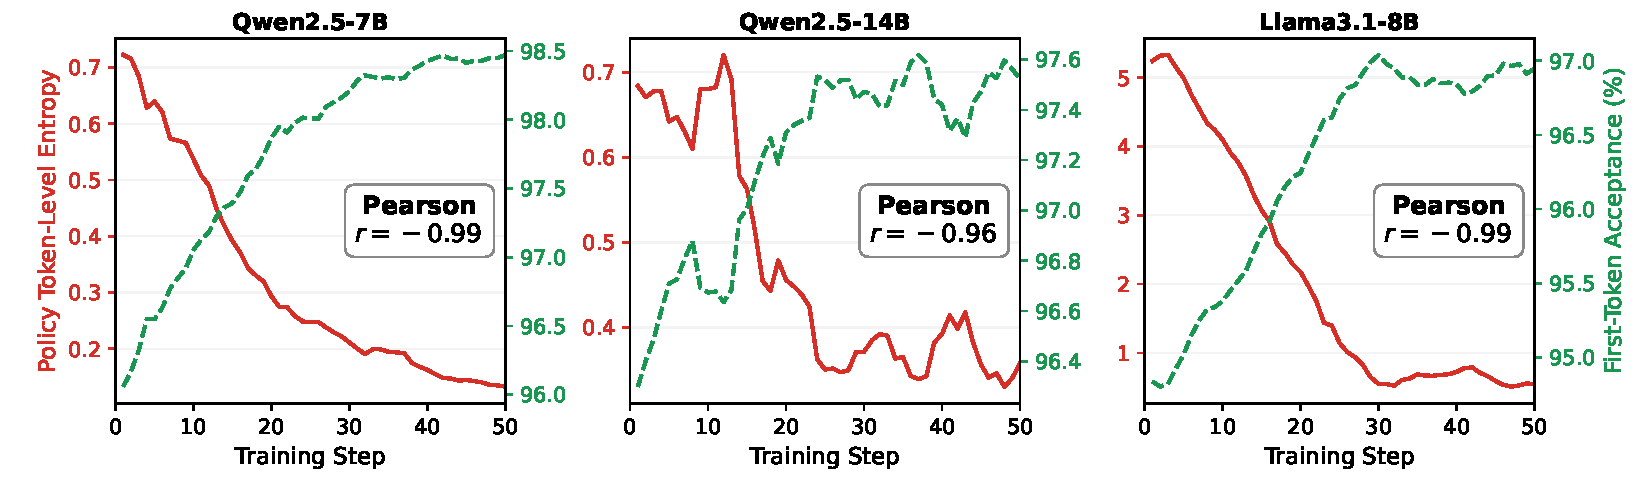
\includegraphics[width=\textwidth]{figures/appendix_motivation_entropy_acc.pdf}
    \caption{
    Policy sharpening improves quantized drafter alignment.
    As target-policy entropy decreases, first-token acceptance of the RTN W4 drafter increases across models.
    }
    \label{fig:appendix_entropy_acceptance}
\end{figure}

\begin{figure}[t]
    \centering
    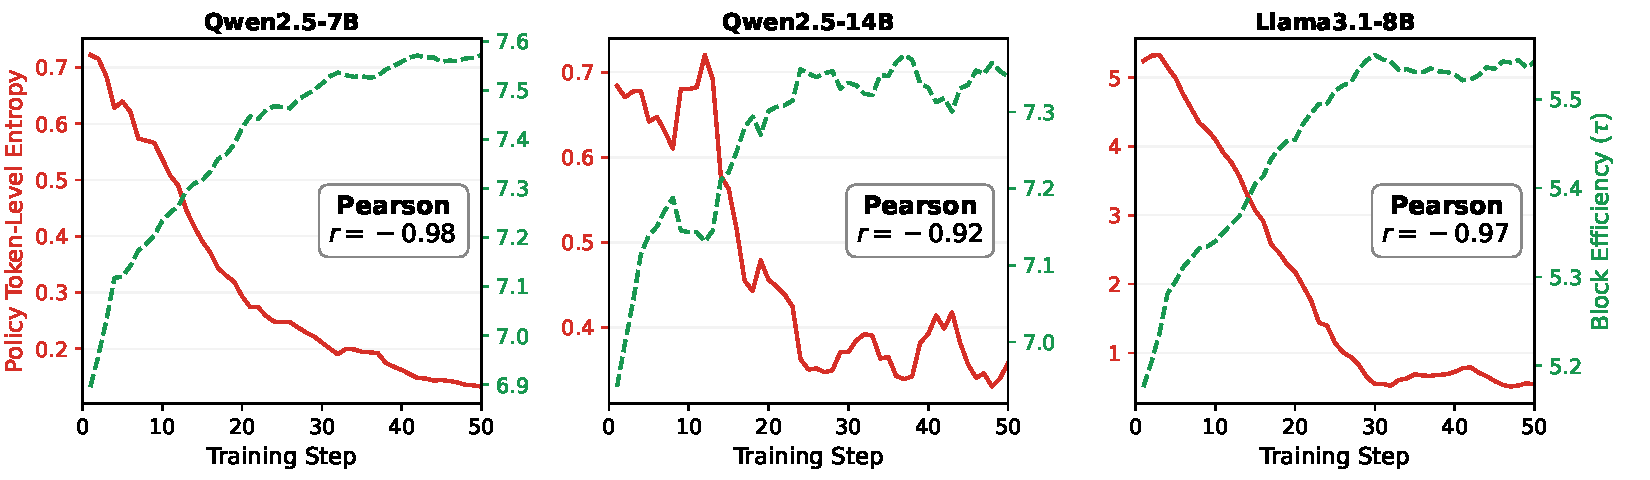
\includegraphics[width=\textwidth]{figures/appendix_motivation_entropy_mal.pdf}
    \caption{
    Policy sharpening improves quantized drafter alignment.
    As target-policy entropy decreases, block efficiency $\tau$ of the RTN W4 drafter increases across models.
    }
    \label{fig:appendix_entropy_mal}
\end{figure}

We analyze how RL training affects quantized self-drafting under a fixed SD configuration, without the regime-aware toggle or adaptive draft-length control.
At each training step, we construct the drafter by applying vanilla round-to-nearest (RTN) 4-bit quantization to the current target model, and use this quantized copy to propose drafts with a fixed draft length.
We measure two quantities: first-token acceptance rate, defined as the fraction of SD iterations in which the first drafted token is accepted by the full-precision target model, and block efficiency $\tau$, defined as the average number of target-distributed tokens produced per SD iteration.
The former directly reflects local drafter--target alignment at the current prefix, while the latter captures the resulting effectiveness of each SD block.

\Cref{fig:appendix_entropy_acceptance} shows the target-policy entropy and first-token acceptance rate over training for Qwen2.5-7B, Qwen2.5-14B, and Llama3.1-8B-Instruct.
Across all three models, RL training reduces policy entropy while first-token acceptance steadily increases, with strong negative Pearson correlations ranging from $-0.96$ to $-0.99$.
\Cref{fig:appendix_entropy_mal} shows that block efficiency follows the same trend, with Pearson correlations ranging from $-0.92$ to $-0.98$.
These results suggest that RL post-training sharpens the target distribution, making small quantization-induced perturbations less likely to change accepted draft tokens and thereby improving block efficiency over training.
